\subsection{Реализция серверной части.}

\subsubsection{Структура решения.}

\textbf{Структура Controllers} изображена на рисунке \ref{fig:Controllers}:
\begin{figure}[!h]
    \centering
    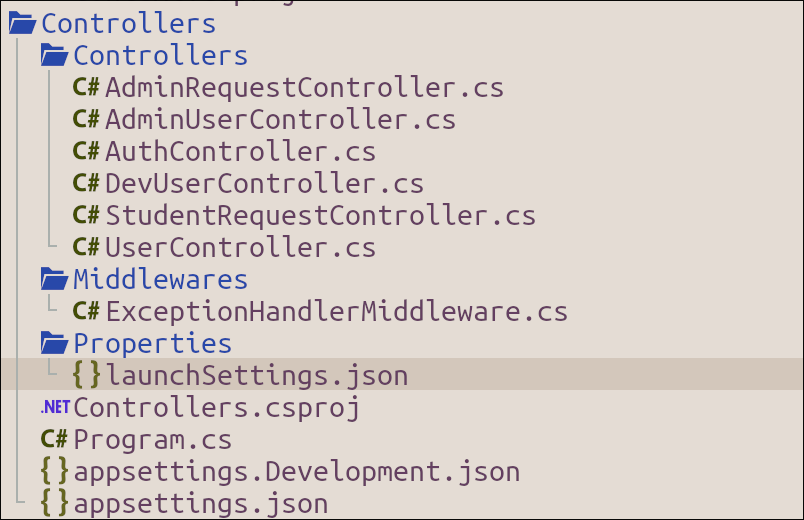
\includegraphics[width = 0.7\textwidth]{imgs/Controllers.png}
    \caption{Схема структуры Controllers}
    \label{fig:Controllers}
\end{figure}

\textbf{Структура Services} изображена на рисунке \ref{fig:Services}:
\newpage
\begin{figure}[!h]
    \centering
    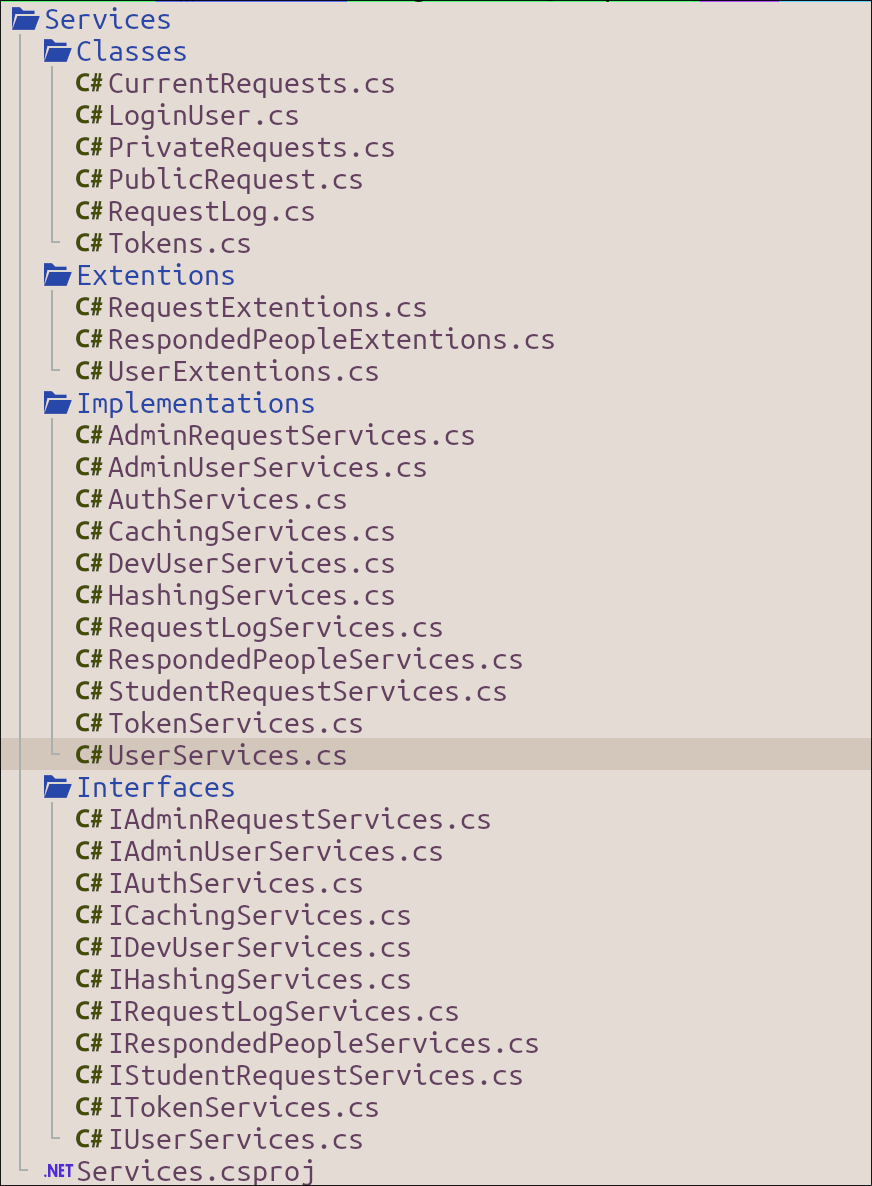
\includegraphics[width = 0.63\textwidth]{imgs/Services.png}
    \caption{Схема структуры Services}
    \label{fig:Services}
\end{figure}

\textbf{Структура Context} изображена на рисунке \ref{fig:Context}:
\begin{figure}[!h]
    \centering
    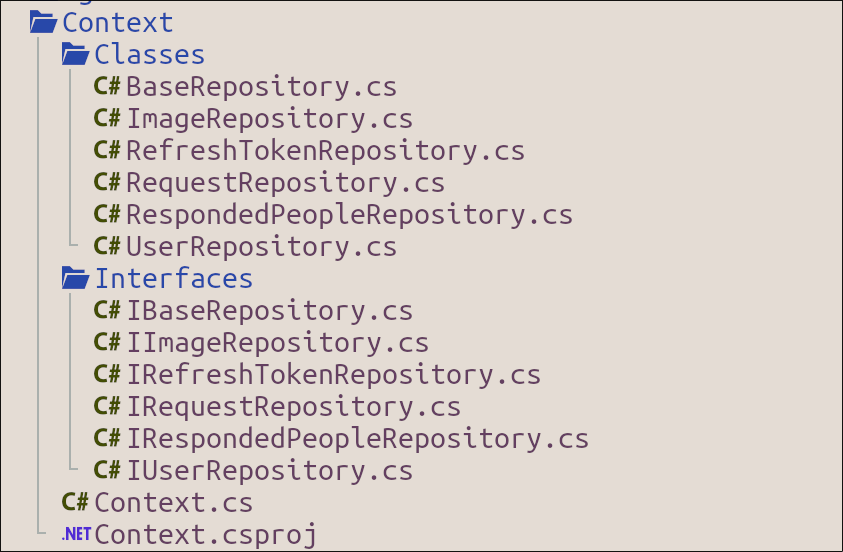
\includegraphics[width = 0.65\textwidth]{imgs/Context.png}
    \caption{Схема структуры Context}
    \label{fig:Context}
\end{figure}

\textbf{Структура Database} изображена на рисунке \ref{fig:Database}:
\begin{figure}[!h]
    \centering
    \includegraphics[width = 0.65\textwidth]{imgs/Database.png}
    \caption{Схема структуры Controllers}
    \label{fig:Database}
\end{figure}

\textbf{Схема структуры серверной части} изображена на рисунке \ref{fig:ProjectStructure}:
\begin{figure}[!h]
    \centering
    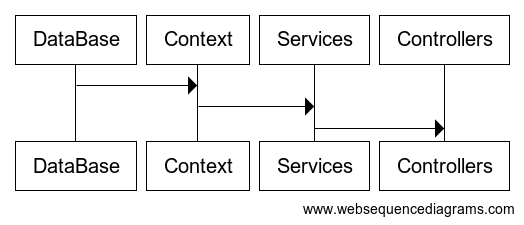
\includegraphics[width = 0.65\textwidth]{imgs/ProjectStruct.png}
    \caption{Схема структуры серверной части}
    \label{fig:ProjectStructure}
\end{figure}

\subsubsection{Реализация JWT.}
% NOTE: JWT
Данная реализация JWT состоит из двух токенов:
\begin{enumerate}
	\item{\textbf{Access Token} --- короткоживущий (5 минут) токен, содержит основные claims (Id, имя пользователя, роль).}
	\item{\textbf{Refresh Token} --- долгоживущий (24 часа) токен, содержит аналогичные claims, но с дополнительным Jti (уникальный идентификатор).}
\end{enumerate}

Access Token используется для аутентификации пользователя и получения разрешения на доступ к защищенному ресурсу. Refresh Token используется для обновления Access Token в случае его устаревания. Так же для предотвращения использования украденных валидных Refresh Token, данный токен сохраняется в базе данных и удаляется при выходе пользователя из системы или повторном входе, что обеспечивает его недействительность и исключает возможность повторного применения после завершения сессии.

% NOTE: Генерация токенов:
\textbf{Генерация токенов:} По данным пользователя генерируются токены с учетом их времени жизни и соответствующими секретным ключам.
\begin{minted}{cs}
    private string GenerateAccessToken(User user, string secretKey)
    {
        var claims = GenerateClaimsAccess(user);
        var token = GenerateToken(claims, secretKey, accessTokenTime);
        return new JwtSecurityTokenHandler().WriteToken(token);
    }

    private string GenerateRefreshToken(User user, string secretKey)
    {
        var claims = GenerateClaimsRefresh(user);
        var token = GenerateToken(claims, secretKey + "sault", refreshTokenTime);
        return new JwtSecurityTokenHandler().WriteToken(token);
    }
\end{minted}

% NOTE: Валидация Refresh Token 
\textbf{Валидация Refresh Token:} Если Refresh Token валиден, то возвращает Ok, если просрочен, то Ok с описанием, что время жизни токена истекло, иначе BadRequest с описанием, что токен невалидный.
\begin{minted}{cs}
    private BaseResponse<Tokens> ValidateRefreshToken(string token, string secretKey)
    {
        var tokenHandler = new JwtSecurityTokenHandler();
        var validationParameters = new TokenValidationParameters
        {
            ValidateIssuerSigningKey = true,
            IssuerSigningKey = new SymmetricSecurityKey(Encoding.ASCII.GetBytes(secretKey + "sault")),
            ValidateIssuer = false,
            ValidateAudience = false,
            ClockSkew = TimeSpan.Zero
        };
        try
        {
            // Проверка подписи JWT
            tokenHandler.ValidateToken(token, validationParameters, out _);
            return BaseResponse<Tokens>.Ok();
        }
        catch (SecurityTokenExpiredException ex)
        {
            return BaseResponse<Tokens>.Ok(description: "Token expired");
        }
        catch (SecurityTokenException ex)
        {
            return BaseResponse<Tokens>.BadRequest(description: "Tokens not valid");
        }
    }
\end{minted}

% NOTE: Обновление токенов:
\textbf{Обновление токенов:} Обновление токенов состоит из нескольких этапов:
\begin{itemize}
	\item{Проверка токена на валидность;}
\end{itemize}
\begin{minted}{cs}
    public async Task<IBaseResponse<Tokens>> RefreshToken(string oldRefreshToken, string secretKey)
    {
        BaseResponse<Tokens> response = ValidateRefreshToken(oldRefreshToken, secretKey);

        if (response.StatusCode == StatusCodes.BadRequest)
        {
            return response;
        }
\end{minted}

\begin{itemize}
	\item{Перенос данных из Refresh Token в User для дальнейшего создания Access Token по этим данным:}
\end{itemize}
\begin{minted}{cs}
        var oldToken = new JwtSecurityTokenHandler().ReadJwtToken(oldRefreshToken);
        User user = new User();

        user.Id = Convert.ToInt32(oldToken.Claims.First(
                    claim => claim.Type == JwtRegisteredClaimNames.Sub
                    ).Value);
        user.Name = Convert.ToString(oldToken.Claims.First(
                    claim => claim.Type == JwtRegisteredClaimNames.Name
                    ).Value);
        user.Role = Convert.ToString(oldToken.Claims.First(
                    claim => claim.Type == ClaimTypes.Role
                    ).Value);
\end{minted}

\begin{itemize}
	\item{Проверка на нахождение Refresh Token в базе данных (если его там нет, то считаем недействительным):}
\end{itemize}
\begin{minted}{cs}
        var oldRefreshDB = await _RefreshTokenRepository.FirstOrDefaultAsync(token => token.Token == oldRefreshToken);
        if (oldRefreshDB == null)
        {
            response = BaseResponse<Tokens>.NotFound();
            return response;
        }
\end{minted}

\begin{itemize}
	\item{Обновление Refresh Token, если токен не просрочен, то оставляем старый, иначе создаем новый и перезаписываем старый в базе данных:}
\end{itemize}
\begin{minted}{cs}
        var oldTokenDB = new JwtSecurityTokenHandler().ReadJwtToken(oldRefreshDB.Token);

        string refreshToken = oldRefreshDB.Token;
        if (response.Description == "Token expired")
        {
            await _RefreshTokenRepository.Delete(oldRefreshDB);

            // Пересоздаем oldRefreshToken, если тот истек
            refreshToken = GenerateRefreshToken(user, secretKey);

            RefreshToken saveRefreshToken = new RefreshToken
            {
                Id = user.Id,
                Token = refreshToken
            };
            await _RefreshTokenRepository.Create(saveRefreshToken);
        }
\end{minted}

\begin{itemize}
	\item{Создание Access Token по данным извлеченным из Refresh Token:}
\end{itemize}
\begin{minted}{cs}
        string accessToken = GenerateAccessToken(user, secretKey);
        response = BaseResponse<Tokens>.Ok(new Tokens
        {
            AccessToken = accessToken,
            RefreshToken = refreshToken
        });
        return response;
    }
\end{minted}

% NOTE: Удаление Refresh Token из бд: 
\textbf{Удаление Refresh Token из бд:} Удаление Refresh Token из базы данных по Id пользователя, если токен не найден в базе данных, то возвращает NoContent, иначе Ok
\begin{minted}{cs}
    public async Task<IBaseResponse> DeleteRefreshToken(int userId)
    {
        BaseResponse response;

        var refreshToken = await _RefreshTokenRepository.FirstOrDefaultAsync(token => token.Id == userId);

        if (refreshToken == null)
        {
            response = BaseResponse.NoContent();
            return response;
        }
        await _RefreshTokenRepository.Delete(refreshToken);

        response = BaseResponse.Ok();
        return response;
    }
\end{minted}

Для передачи токенов в клиентскую часть приложения используется класс Tokens состоящий из двух полей:

\begin{minted}{cs}
public class Tokens
{
    public string AccessToken { get; set; }
    public string RefreshToken { get; set; }
}
\end{minted}

Рассмотрим получение токенов при входе в аккаунт. Для этого необходимо отправить JSON изображенный на рисунке \ref{fig:LoginInput}:

\begin{figure}[!h]
    \centering
    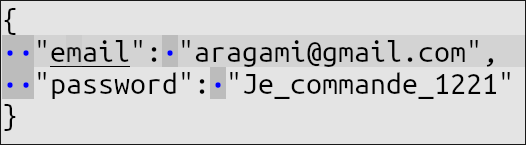
\includegraphics[width = 0.7\textwidth]{imgs/LoginInput.png}
    \caption{Пример отправленного JSON при входе в аккаунт}
    \label{fig:LoginInput}
\end{figure}

В ответ на это приходит JSON изображенный на рисунке \ref{fig:LoginOutput}:

\newpage
\begin{figure}[!h]
    \centering
    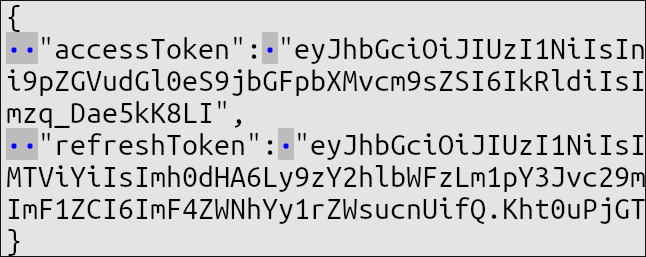
\includegraphics[width = 0.7\textwidth]{imgs/LoginOutput.png}
    \caption{Пример полученного JSON при входе в аккаунт}
    \label{fig:LoginOutput}
\end{figure}

Вся оставшаяся реализация токенов находится в отдельном классе: TokenServices. Полный код для TokenServices находится в приложении \ref{app:TokenServices}

\subsubsection{Реализация ленты запросов, для администраторов и пользователей.}

Рассмотрим реализацию ленты запросов для администраторов и пользователей. Лента запросов позволяет администраторам и пользователям видеть список запросов с определнными данными в зависимости от роли. Например информация о том, кто создал или поменял запрос доступна только администраторам.

% NOTE: Лента админов
\textbf{Лента админов:} Если есть запросы и откликнувшиеся на них люди, то объединяем их в \mintinline{cs}{List<PrivateReqest>} и далее выводим.
\begin{minted}{cs}
				// Получаем откликнувшихся на запросы
        var respondedPeople = await _RespondedPeopleRepository.GetAll();

        List<PrivateRequest> requests;

        if (respondedPeople != null && respondedPeople.Count > 0)
        {
            // Ищем в БД
            requests = await _RequestRepository
                .GetQueryable()
                .Select(request => new PrivateRequest(request, respondedPeople)) // Преобразуем в PrivateRequest с откликнувшимися людьми
                .ToListAsync();
        }
        else
        {
            // Ищем в БД
            requests = await _RequestRepository
                .GetQueryable()
                .Select(request => new PrivateRequest(request)) // Преобразуем в PrivateRequest без откликнувшихся людей
                .ToListAsync();
        }
\end{minted}

\textbf{Лента пользователей:}  Если есть запросы и откликнувшиеся на них люди, то объединяем их в \mintinline{cs}{List<PublicRequest>} и далее выводим.
\begin{minted}{cs}
				// Получаем откликнувшихся на запросы
        var respondedPeople = await _RespondedPeopleRepository.GetAll();

        List<PublicRequest> requests;

        if (respondedPeople != null && respondedPeople.Count > 0)
        {
            // Ищем в БД
            requests = await _RequestRepository
                .GetQueryable()
                .Select(request => new PublicRequest(request, respondedPeople)) // Преобразуем в PublicRequest с откликнувшимися людьми
                .ToListAsync();
        }
        else
        {
            // Ищем в БД
            requests = await _RequestRepository
                .GetQueryable()
                .Select(request => new PublicRequest(request)) // Преобразуем в PublicRequest без откликнувшихся людей
                .ToListAsync();
        }
\end{minted}

Как можно заметить, в реализации лент запросов, при получении списка сущности \mintinline{cs}{Request} из базы данных, происходит приведение сущности \mintinline{cs}{Request} к классу \mintinline{cs}{PublicRequest} или \mintinline{cs}{PrivateRequest} в зависимости от того, какие данные можно отобразить в ленте для данной роли. А так же при данном преобразовании добавляются к каждому запросу записавшиеся на него люди, если они есть.

Пример ленты пользователя изображен на рисунке \ref{fig:PublicFeed}:

\newpage
\begin{figure}[!h]
    \centering
    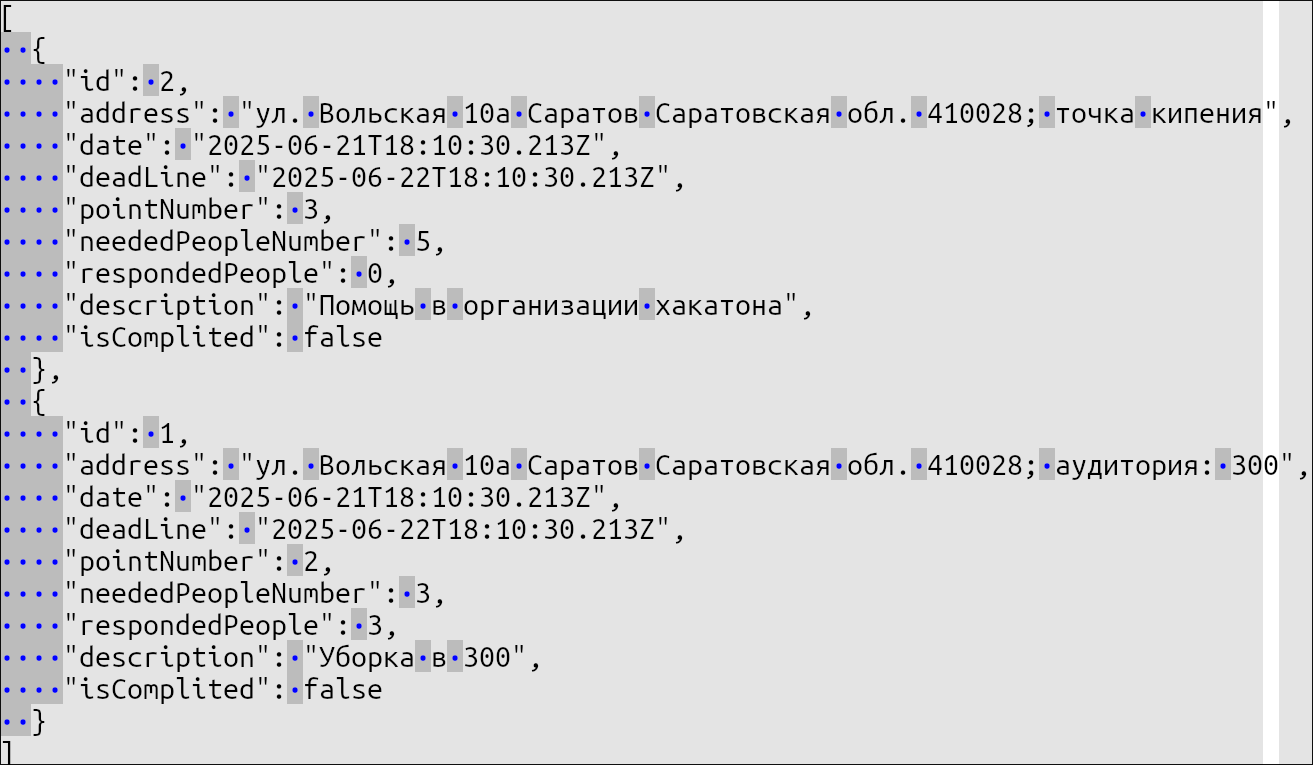
\includegraphics[width = 0.75\textwidth]{imgs/PublicFeed.png}
    \caption{Пример ленты пользователя}
    \label{fig:PublicFeed}
\end{figure}

Пример ленты администратора изображен на рисунке \ref{fig:AdminFeed}:

\begin{figure}[!h]
    \centering
    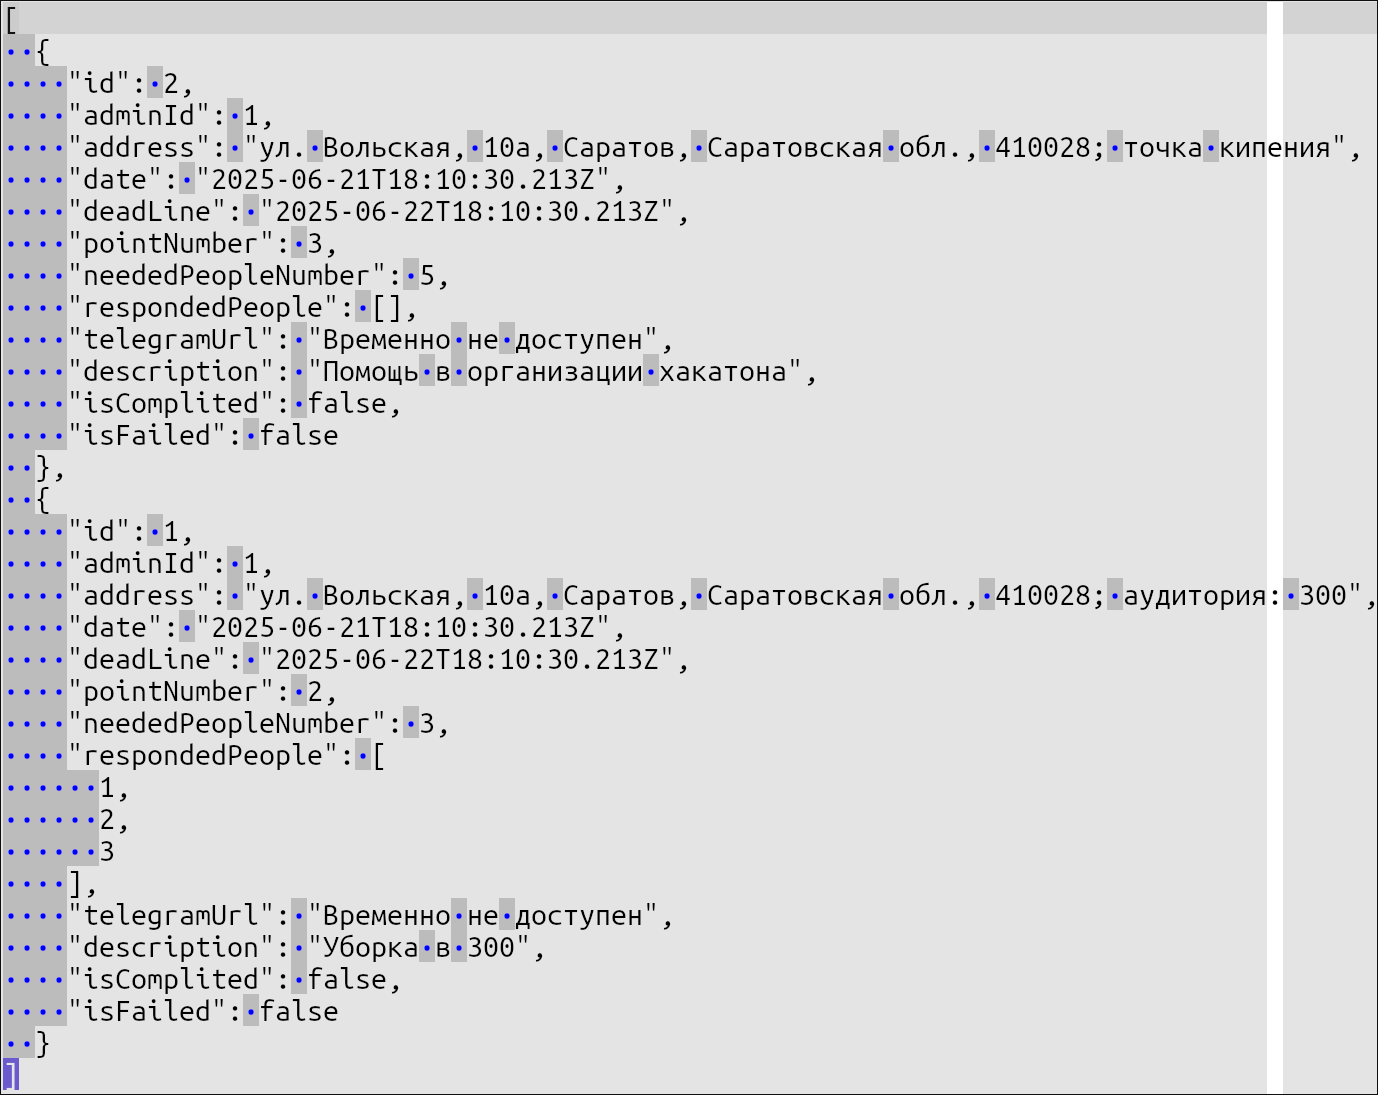
\includegraphics[width = 0.7\textwidth]{imgs/AdminFeed.png}
    \caption{Пример ленты администратора}
    \label{fig:AdminFeed}
\end{figure}
Полная реализация находится в классах AdminRequestServices и StudentRequestServices, их можно найти в приложении \ref{app:Others}

\subsubsection{Реализация возможности записаться на запрос и отписаться с запроса.}

\textbf{Добавление пользователя к запросу:} добавление пользователя к запросу состоит из нескольких этапов:
\begin{itemize}
	\item{Ищем запрос в БД:}
\end{itemize}
\begin{minted}{cs}
    public async Task<IBaseResponse> AssignMe(int requestId)
    {
        BaseResponse response;

        var request = await _RequestRepository.FirstOrDefaultAsync(rq => rq.Id == requestId);

        // Если запроса нет
        if (request == null)
        {
            // NotFound (404)
            response = BaseResponse.NotFound("Request not found");
            return response;
        }

\end{minted}

\begin{itemize}
	\item{Если запрос найден, ищем откликнувшихся на данный запрос:}
\end{itemize}
\begin{minted}{cs}
        var respondedPeople = await _RespondedPeopleRepository
            .Where(rp => rp.RequestId == requestId)
            .ToListAsync();
\end{minted}

\begin{itemize}
	\item{Если остались места и студент не откликался на запрос, то добавляем его в откликнувшихся:}
\end{itemize}
\begin{minted}{cs}
        if (respondedPeople.Count < request.NeededPeopleNumber)
        {
            // Получаем Id откликнувшегося студента из токена
            int myId = _UserServices.GetMyId();
            if (respondedPeople.Where(rp => rp.UserId == myId).Any())
            {
                // BadRequest (400)
                response = BaseResponse.BadRequest("Already added");
                return response;
            }

            // Добавляем студента к откликнувшимся
            RespondedPeople newRP = new RespondedPeople();
            newRP.RequestId = requestId;
            newRP.UserId = myId;
            await _RespondedPeopleRepository.Create(newRP);

            // NoContent (204)
            response = BaseResponse.NoContent("Successed");
            return response;
        }
        // BadRequest (400)
        response = BaseResponse.BadRequest("No more places");
        return response;
    }
\end{minted}


\textbf{Удаление пользователя из откликнувшихся на запроc:} удаление пользователя из откликнувшихся на запроc состоит из нескольких этапов:
\begin{itemize}
	\item{Ищем запрос в БД и если запрос найден, то ищем откликнувшихся на данный запрос:}
\end{itemize}
\begin{minted}{cs}
        var request = await _RequestRepository.FirstOrDefaultAsync(rq => rq.Id == requestId);

        if (request == null)
        {
            // NotFound (404)
            response = BaseResponse.NotFound("Request not found");
            return response;
        }

        // Ищем откликнувшихся на запрос
        var respondedPeople = await _RespondedPeopleRepository
            .Where(rp => rp.RequestId == requestId)
            .ToListAsync();

\end{minted}

\begin{itemize}
	\item{Получаем Id пользователя из токена и ищем его в списке откликнувшихся на запрос:}
\end{itemize}
\begin{minted}{cs}
        int myId = _UserServices.GetMyId();
        // Ищем отклик студента
        RespondedPeople deleteRP = respondedPeople
            .FirstOrDefault(rp => (rp.UserId == myId && rp.RequestId == request.Id));

\end{minted}

\begin{itemize}
	\item{Если студент уже откликался, то удаляем его из откликнувшихся на запрос иначе выдаем BadRequest (400), так как пользователь не откликался:}
\end{itemize}
\begin{minted}{cs}
        if (deleteRP != null)
        {
            await _RespondedPeopleRepository.Delete(deleteRP);
            // NoContent (204)
            response = BaseResponse.NoContent("Successed");
            return response;
        }
        // BadRequest (400)
        response = BaseResponse.BadRequest("Was not assigned");
        return response;
\end{minted}

\subsubsection{Реализация начисления очков за выполненный запрос.}

Рассмотрим реализацию начисления очков за выполненный запрос. В данном действии происходит:
\begin{itemize}
	\item{Начисление очков за выполнение запроса}
	\item{Закрытие запроса как выполненного}
\end{itemize}

\textbf{Начисление очков за выполненный запрос:} Начисляем очки за выполненный запрос состоит из нескольких этапов:

\begin{itemize}
	\item{Ищем запрос в БД и проверяем его наличие и возможность закрыть его как выполненный, то есть проверяем:
			\begin{itemize}
				\item{Если не имеет запрос нужное количество мест для данного количества Id пользователей, то возвращаем UnprocessableContent(422):}
				\item{Если запрос уже выполнен, то возвращаем BadRequest(400):}
				\item{Если запрос провален, то возвращаем BadRequest(400):}
			\end{itemize}
		}
\end{itemize}
\begin{minted}{cs}
        var request = await _RequestRepository.FirstOrDefaultAsync(rq => rq.Id == requestId);
        if (request == null)
        {
            response = BaseResponse.NotFound("Request not found");
            return response;
        }
        if (usersId.Count > request.NeededPeopleNumber)
        {
            response = BaseResponse.UnprocessableContent("Number of Ids is more than necessary");
            return response;
        }
        if (request.IsComplited == true)
        {
            response = BaseResponse.BadRequest("Request is already Completed");
            return response;
        }
        if (request.IsFailed == true)
        {
            response = BaseResponse.BadRequest("Request is already Failed");
            return response;
        }
\end{minted}

\begin{itemize}
	\item{Вызываем метод начисления очков за выполненный запрос:}
\end{itemize}
\begin{minted}{cs}
        response = await PointsPerRequest(request.PointNumber, usersId);
\end{minted}

\textbf{Реализация метода начисления очков за выполненный запрос:}
\begin{itemize}
	\item{Находим всех пользователей из списка Id и если они все существуют, то начисляем им очки за выполнение запроса и увеличиваем количество завершенных запросов пользователя:}
\end{itemize}
\begin{minted}{cs}
    private async Task<IBaseResponse> PointsPerRequest(int points, List<int> usersId)
    {
        BaseResponse response;
        List<User> users = new List<User>();
        User user;

        for (int i = 0; i < usersId.Count; i++)
        {
            user = await _UserRepository.FirstOrDefaultAsync(us => us.Id == usersId[i]);

            if (user == null)
            {
                response = BaseResponse.NotFound("User is not found");
                return response;
            }

            user.Points += points;
            user.FinishedRequests += 1;
        }
\end{minted}

\begin{itemize}
	\item{Если все пользователи существуют, то начисляем им очки за выполнение запроса:}
\end{itemize}
\begin{minted}{cs}
        for (int i = 0; i < users.Count; i++)
        {
            await _UserRepository.Update(users[i]);
        }
        response = BaseResponse.NoContent();
        return response;
    }
\end{minted}

\begin{itemize}
	\item{Если все пользователи существовали, то отмечаем запрос как выполненный, сохраняем изменение запроса в бд и логируем изменение запроса в файл, иначе возвращаем NotFound (404):}
\end{itemize}
\begin{minted}{cs}
        if (response.StatusCode == DataBase.StatusCodes.NotFound)
        {
            return response;
        }
        request.IsComplited = true;

        await _RequestRepository.Update(request);

        RequestLog log = new RequestLog(0, request.AdminId, request.Id, $"Request MarkAsCompleted");
        _RequestLogServices.AppendLogToFile(log);
\end{minted}

\subsubsection{Реализация логирования изменений запроса администратором.}

Рассмотрим реализацию логирования изменений запроса администратором. Она нужна для отслеживания изменений в запросе и позволяет легко увидеть нежелательные изменения в запросе, а так же позволит быстро определить администратора, который сделал нежелательные правки запроса.

\textbf{Создание пути к файлу:} Создаем путь к файлу по Id запроса:
\begin{minted}{cs}
    private string CreatePathToLog(int requestId)
    {
        string fileName = TemplateLogFileName + requestId.ToString() + ".log";
        string pathToLog = Path.Combine(LogsDir, fileName);
        return pathToLog;
    }
\end{minted}

\textbf{Добавление лога в файл:} Добавляем переданный в метод лог в файл последней строкой:
\begin{itemize}
	\item{Создаем путь к файлу для записи лога}
\end{itemize}
\begin{minted}{cs}
    public void AppendLogToFile(RequestLog log)
    {
        string pathToLog = CreatePathToLog(log.RequestId);
\end{minted}
\begin{itemize}
	\item{Находим последний log Id и задаем новый log Id для новой записи}
\end{itemize}
\begin{minted}{cs}
        RequestLog lastLog = ReadLastLogFromFile(pathToLog);
        log.Id = lastLog.Id + 1;
\end{minted}

\begin{itemize}
	\item{Создаем файл по пути из pathToLog, если он еще не существует}
\end{itemize}
\begin{minted}{cs}
        EnsureFileExist(pathToLog);
\end{minted}

\begin{itemize}
	\item{Создаем строку для лога и записываем ее в файл}
\end{itemize}
\begin{minted}{cs}
        string newLog = $"{log.Id}, {log.AdminId}, {log.RequestId}, {AddEscaping(log.Action)}, {log.Date:O}";

        File.AppendAllText(pathToLog, newLog + Environment.NewLine);
    }
\end{minted}

\textbf{Парсинг лога из файла:} Парсинг строки лога из файла в класс RequestLog:
\begin{itemize}
	\item{Создаем массив строк из строки, в которой данные разделены запятой}
	\item{Парсим массив строк в класс RequestLog, где каждый элемент массива это отдельное поле RequestLog}
\end{itemize}
\begin{minted}{cs}
    private static RequestLog ParseLogLine(string logLine)
    {
        var parts = logLine.Split(",");
        return new RequestLog(
                int.Parse(parts[0]),
                int.Parse(parts[1]),
                int.Parse(parts[2]),
                RemoveEscaping(parts[3]),
                DateTime.Parse(parts[4])
        );
    }
\end{minted}

\textbf{Чтение логов из файла:} Чтение всех логов запроса по его Id, возвращает List из логов, если файл существует, иначе возвращает пустой List
\begin{minted}{cs}
    public List<RequestLog> ReadAllLogsFromFile(int requestId)
    {
        // Путь до файла
        string pathToLog = CreatePathToLog(requestId);

        if (!File.Exists(pathToLog))
        {
            return new List<RequestLog>();
        }

        return File.ReadAllLines(pathToLog)
            .Where(line => !string.IsNullOrEmpty(line))
            .Select(ParseLogLine)
            .ToList();
    }
\end{minted}

\textbf{Удаление файла лога:} Удаляем файл по Id запроса, если он существует:
\begin{minted}{cs}
    public void DeleteLogFile(int requestId)
    {
        // Путь до файла
        string pathToLog = CreatePathToLog(requestId);

        if (File.Exists(pathToLog))
        {
            File.Delete(pathToLog);
        }
    }
\end{minted}

Полная реализация находится в классе RequestLogServices.В примере кода ниже приведены лишь некоторые методы из класса. Весь код можно найти в приложении \ref{app:Others}.

\subsubsection{Реализация повшения до администратора и понижения до пользователя.}

\textbf{Повшение до администратора:} Выдает роль администратора по почте пользователя, если он является студентом.
\begin{minted}{cs}
    public async Task<IBaseResponse> PromoteToAdmin(string userEmail)
    {
        BaseResponse response;
        var user = await _UserRepository.FirstOrDefaultAsync(us => us.Email == userEmail);

        if (user == null)
        {
            response = BaseResponse.NotFound("User not found");
            return response;
        }
        if (user.Role != "Student")
        {
            response = BaseResponse.BadRequest("User is not Student");
            return response;
        }
        user.Role = "Admin";
        await _UserRepository.Update(user);
        response = BaseResponse.NoContent();
        return response;
    }
\end{minted}

\textbf{Понижение до пользователя:} Выдает роль пользователя по почте пользователя, если он является администратором.
\begin{minted}{cs}
    public async Task<IBaseResponse> DemoteToStudent(string userEmail)
    {
        BaseResponse response;
        var user = await _UserRepository.FirstOrDefaultAsync(us => us.Email == userEmail);

        if (user == null)
        {
            response = BaseResponse.NotFound("User not found");
            return response;
        }
        if (user.Role == "Admin")
        {
            user.Role = "Student";
            await _UserRepository.Update(user);
            response = BaseResponse.NoContent();
            return response;
        }
        response = BaseResponse.BadRequest("User is not Admin");
        return response;
    }
\end{minted}
